% =========================
% Course Notes Template
% main.tex
% =========================
\documentclass[11pt]{article}

% ----- Page layout -----
\usepackage[margin=0.9in]{geometry}
\usepackage{setspace}
\setstretch{1.08}
\setcounter{secnumdepth}{0}

% ----- Fonts (good default) -----
\usepackage[T1]{fontenc}
\usepackage{lmodern}

% ----- Math -----
\usepackage{amsmath, amssymb, amsthm, mathtools}
\usepackage{bm} % bold math symbols
\usepackage{nicematrix}

% ----- Figures / tables -----
\usepackage{graphicx}
\usepackage{subcaption}
\usepackage{booktabs}

% Put images in a folder named "figures/"
\graphicspath{{imgs/}}

% ----- Colors, links, and references -----
\usepackage{xcolor}
\usepackage[hidelinks]{hyperref}
\hypersetup{colorlinks=true,linkcolor=blue,urlcolor=blue}
\usepackage[nameinlink, capitalize]{cleveref}

% ----- Lists -----
\usepackage{enumitem}
\setlist[itemize]{topsep=4pt, itemsep=2pt}
\setlist[enumerate]{topsep=4pt, itemsep=2pt}

% ----- Code blocks (optional) -----
\usepackage{listings}
\lstset{
  basicstyle=\ttfamily\small,
  breaklines=true,
  frame=single,
  numbers=left,
  numberstyle=\tiny,
  xleftmargin=2em,
  framexleftmargin=1.5em
}

% ----- Pseudo Code -----
\usepackage{algorithm}
\usepackage{algpseudocode}
\algnewcommand{\Input}{\State \textbf{Input:}}
\algnewcommand{\Output}{\State \textbf{Output:}}

% ----- Theorem-like environments -----
\usepackage{cancel}
\theoremstyle{definition}
\newtheorem{definition}{Definition}[section]
\newtheorem{example}{Example}[section]

\theoremstyle{plain}
\newtheorem{theorem}{Theorem}[section]
\newtheorem{lemma}{Lemma}[section]

\theoremstyle{remark}
\newtheorem{remark}{Remark}[section]

% ----- Handy macros (edit as you like) -----
\newcommand{\R}{\mathbb{R}}
\newcommand{\dd}{\,\mathrm{d}}
\newcommand{\pd}[2]{\frac{\partial #1}{\partial #2}}
\newcommand{\grad}{\nabla}
\newcommand{\divg}{\nabla\cdot}
\newcommand{\curl}{\nabla\times}

% ----- Title info -----
\title{\textbf{Uncertainty Quantification - Homework 2}}
\author{Leonid Scott}

\begin{document}

\maketitle

% =========================
\section{Problem Setting}
This submission models the following 1D diffusion equation with both Polynomial Chaos Expansions (PCE) and Karhunen-Loève Expansions + Gaussian Processes (KLE-GP):

\begin{equation}
-\frac{d}{dx}\left( \nu(x,\xi) \frac{du}{dx} \right) = s(x) \\
,x \in [0,1]. B.C.s: u(0) = u(1) = 0
\end{equation}

\noindent Where $s(x) = \sin(\pi x)$, and $v(x,xi) = v_0 (1 + \alpha \tanh(\sum_{i=1}^5 \xi_i \sin(i \pi x)))$.

\noindent $v_0 = 0.1$, and $\alpha = 0.5$. $\vec{\xi} \in \mathbb{R}^5$, $\xi_i \text{ are } i.i.d$, and$\xi_i \sim N(0,1)$.


\section{Numerical Scheme of Model}
Equation (1) is modelled using a 2nd order finite difference scheme across a uniformly spaced mesh from $x=0$, and $x=1$. The mesh is discrtized into $N$ points, each spaced $\Delta x$ apart. Therefore, the discrtized equation for the left hand side of (1) at mesh point $i$ is:
$$
\left. \frac{du}{dx} \right|_i \simeq \frac{u_{i+1/2} - u_{i-1/2}}{\Delta x}
$$
$$
u_{i+1/2} \simeq \nu_{i+1/2} \frac{u_{i+1} - u_i}{\Delta x}, \quad
u_{i-1/2} \simeq \nu_{i-1/2} \frac{u_i - u_{i-1}}{\Delta x}
$$
Subsituted into (1), and rearranged, the discretized form of (1) becomes:
$$
- \nu_{i+1/2} (u_{i+1} - u_i) + \nu_{i-1/2} (u_i - u_{i-1}) = s_i (\Delta x)^2
$$
This scheme can be written as the following linear system:
$$
\mathbf{A} \vec{u} = \vec{s}
$$

$$
\begin{bNiceMatrix}
  [\nu_{i-1/2} + \nu_{i+1/2}] & [-\nu_{i+1/2}] & \cdots \\
  [-\nu_{i-1/2}] & \ddots & \ddots \\
  \vdots & \ddots & \ddots
\end{bNiceMatrix}
\quad
\begin{bNiceMatrix}
  u_0 \\
  \vdots \\
  u_{N-1}
\end{bNiceMatrix}
=
\begin{bNiceMatrix}
  s_0 (\Delta x)^2 \\
  \vdots \\
  s_{N-1} (\Delta x)^2
\end{bNiceMatrix} \\
$$

\noindent Where $\mathbf{A}$ is an $N \times N$ tridiagonal matrix, and boundary conditions are imposed at $u_0$ and $u_{N-1}$. This system can be solved via LU Factorization.

\noindent The following figure shows $u$ with 100 realizations of $\vec{\xi}$.
Qualitatively, it looks like it is in agreement with the posted solution.

\begin{figure}
    \centering
    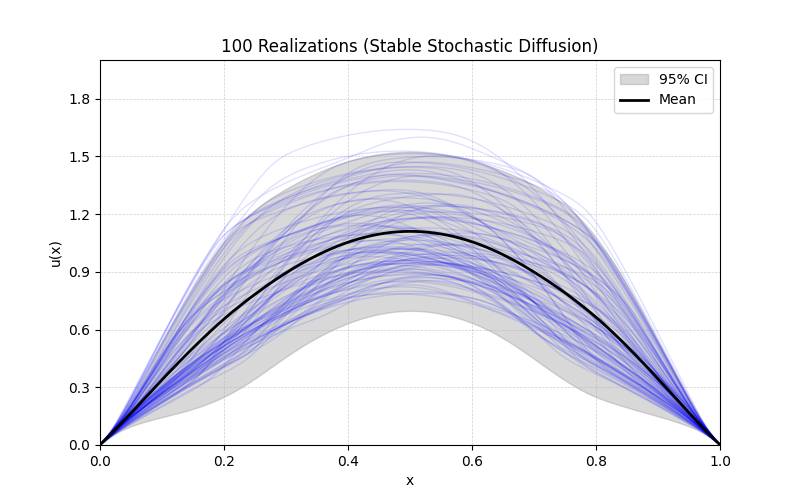
\includegraphics[width=1.0\textwidth]{forward_model.png}
    \label{fig:my_image}
\end{figure}

\section{Polynomial Chaos Expansion Surrogate}

%\section{Appendix 1: Polynomial Chaos Expansion}
A Polynomial Chaos Expansion (PCE) can model a function $f(\vec{x},t;\vec{\xi})$, with independent variables $\vec{x}$, and $t$, and uncertain inputs $\vec{\xi}$. If $\vec{\xi} \in \mathbb{R}^n$, then $n$ can be defined as the \textit{stochastic dimension}, and $f(\vec{x},t;\vec{\xi})$ can be modelled as:
$$
f(\vec{x}, t; \vec{\xi}) \approx \sum_{k=0}^{\text{N\_basis}} c_k(\vec{x},t) \Psi_k(\vec{\xi})
$$
Where:
$$
\text{N\_basis} = \frac{(n + p)!}{n! + p!}
$$
And $p$ is the \textit{Polynomial Order} hyperparameter.

\parskip = \baselineskip
\noindent $\mathbf{\Psi_k(\vec{\xi})}$ - \textbf{Polynomial Basis}: This term represents a collection of polynomials, and is expressed as:
$$
\Psi_k(\vec{\xi}) = \prod_{j=1}^{n} \Psi_{\alpha_j^{(k)}} (\xi_j)
$$
Recall that $n$ is the stochastic dimension. $\Psi_{\alpha_j^{(k)}} (\xi_j)$ is a member of a specific \textit{family} of polynomials depending on the distribution of $\vec{\xi}$:
\begin{itemize}
  \item If $\vec{\xi}$ is \textit{uniformly} distributed, we draw from the \href{https://en.wikipedia.org/wiki/Legendre_polynomials}{Legendre Polynomal Family}.
  \item If $\vec{\xi}$ is distributed according to a \textit{gaussian} distribution, we use the \href{https://en.wikipedia.org/wiki/Hermite_polynomials}{Hermite Polynomal Family}. 
\end{itemize}

\noindent A polynomial of order $k$ in either of these families can be described by a vector of coefficients ranging from the 0th order coefficients up to the $k$th coefficients. However, when we say a polynomial is of order $k$, we mean that the $k^{\text{th}}$ coefficient is 1, and all others are zero.

\noindent Moreover, $\Psi_{\alpha_j^{(k)}}$ is a member of a particular set of a \textit{multi-index} of polynomials.
A multi-index is a set of sets of polynomials.
In particular, it is the set of all sets, each made up of $j$ polynomials, whose total polynomial order equals $k$.
For example:
$$
\Psi_{\alpha_2^{(k)}} = \left\{ (\Psi^0, \Psi^3), (\Psi^3, \Psi^0), (\Psi^1, \Psi^2), (\Psi^2, \Psi^1), (\Psi^2, \Psi^2) \right\}
$$

\noindent $\mathbf{c_k}$ - \textbf{Deterministic Coefficients}: The goal of training a PCE is to find these coefficients. During training, we know $f$ for a range of inputs. Moreover, from the stochastic dimension (enforced by the dimension of $\vec{\xi}$), and user-specified polynomial order, we can calculate $\Psi_k$. All that is left to do is calculate $c_k$.

\noindent We can solve for $c_k$ using either spectral projection or least squares.
While spectral projection takes advantage of the orthogonal nature of our polynomial basis, it's implentation is out of scope here. We instead use a least squares solve to find coefficients.

\subsection{Vector Form of the PCE}
In vector form, a PCE looks like:
$$
\vec{y} = \mathbf{\Psi}(\vec{\xi}) \vec{c}
$$
\subsubsection{Training}
To train a PCE, we create $\text{N\_samples}$ evaluations of $f$, each with a different realization of $\vec{\xi}^{(i)}$. We then populate $\mathbf{\Psi}$ based on: The distribution of $\vec{\xi}$ (Normal or Uniform), a user specified polynomial order $p$, and the stochastic dimension $n$.
Once $\bm{\Psi}$ is calculated, we solve for $\vec{c}$ with a least squares method.

$$
\begin{bmatrix}
f(\vec{x},t ; \vec{\xi}^{(0)}) \\
f(\vec{x},t ; \vec{\xi}^{(1)}) \\
... \\
... \\
f(\vec{x},t ; \vec{\xi}^{(\text{N\_samples} - 1)}) \\
\end{bmatrix}
=
\begin{bmatrix}
\Psi_0(\vec{\xi}^{(0)}) & \Psi_1(\vec{\xi}^{(0)}) & \cdots & \Psi_{\text{N\_basis}}(\vec{\xi}^{(0)}) \\
\Psi_0(\vec{\xi}^{(1)}) & \cdots & \cdots\\
\cdots \\
\Psi_0(\vec{\xi}^{(\text{N\_samples} - 1)}) & \Psi_1(\vec{\xi}^{(\text{N\_samples} - 1)}) & \cdots & \Psi_{\text{N\_basis} - 1}(\vec{\xi}^{(\text{N\_samples} - 1)}) \\
\end{bmatrix}
\begin{bmatrix}
c_0 \\
\cdots \\
c_{\text{N\_basis}}
\end{bmatrix}
$$

\subsubsection{Prediction}
When presented with a novel $\vec{\xi}$ matrix, we populate $\mathbf{\Psi}$ matrix to match the dimension of $\vec{\xi}$, and multiply it against our trained $\vec{c}$ to get an estimate $\tilde{f}(\vec{x},t ; \vec{\xi}_\text{novel})$.

\end{document}